\documentclass[handout]{beamer}
\usepackage{bussproofs}
\usepackage{stmaryrd}

\title{Composable Compcert}
\subtitle{a PLDI paper pitch}
\author{J\'er\'emie Koenig}

% Macros {{{
\newcommand{\EC}{\text{EC}}
\newcommand{\nEC}{\overline{\EC}}
\newcommand{\ECEC}{\EC \Rightarrow \EC}
%\newcommand{\ECEC}{\bar{*} \vee *}
\newcommand{\kw}[1]{\texttt{#1}}
\newcommand{\word}[1]{\mathbf{#1}}
\newcommand{\sys}{\textbf{sys}}
\newcommand{\env}{\textbf{env}}
\newcommand{\ident}{\kw{ident}}
\newcommand{\val}{\kw{val}}
\newcommand{\mem}{\kw{mem}}
\newcommand{\Y}{\mathbf{Y}}
\newcommand{\E}{\mathcal{E}}
%}}}

\setlength{\parskip}{1ex}

\AtBeginSection[]
{
   \begin{frame}
        \tableofcontents[currentsection]
   \end{frame}
}

\begin{document}

\begin{frame}
\titlepage
\end{frame}

\begin{frame}{Bottom line} %{{{
We can build a compositional Compcert
relatively easily if we:
\begin{itemize}
\item give Compcert transition systems a module interface,
  and introduce \emph{external call events},
\item
  consider \emph{abstraction} in the definition of refinement, and
\item
  adapt the notion of \emph{alternating simulation}
  to Compcert.
\end{itemize}
Because it models open systems,
the result can be connected to
other certified components
in a straightforward way.
\end{frame}
%}}}

\section{Semantics in Compcert}

\begin{frame}{Transition Systems} %{{{
The main semantic objects used in Compcert
are labeled transition systems:
\begin{center}
  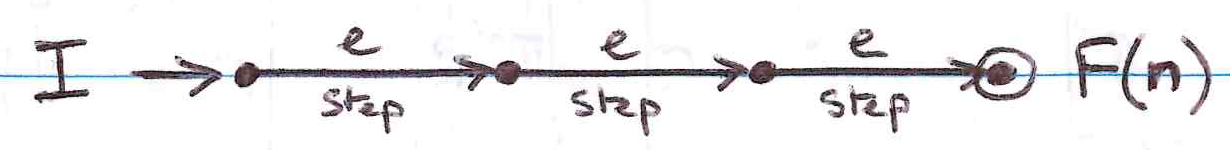
\includegraphics[scale=.65]{figs/trsys}
\end{center}
A labeled transition system is defined by:
\begin{itemize}
  \item a set of states $S$;
  \item a set of initial states $I \subseteq S$;
  \item a transition relation ${\rightarrow} \subseteq S \times \mathbb{E}^* \times S$;
  \item a set of final states $F \subseteq S \times \kw{int}$.
\end{itemize}
\end{frame}
%}}}

\begin{frame}{Behavior} %{{{
The behavior of a transition system is understood as
the set of traces it generates
(together with any associated final result).

Event traces record the program's interaction with the environment.
Compcert events can represent:
\begin{itemize}
  \item system calls with no side-effects;
  \item accesses to volatile variables (cannot read/write non-global pointers).
\end{itemize}
\end{frame}
%}}}

\begin{frame}{Backward Simulations} %{{{
The semantic preservation theorem of Compcert
is expressed in terms of \emph{backward simulations}:
\begin{center}
  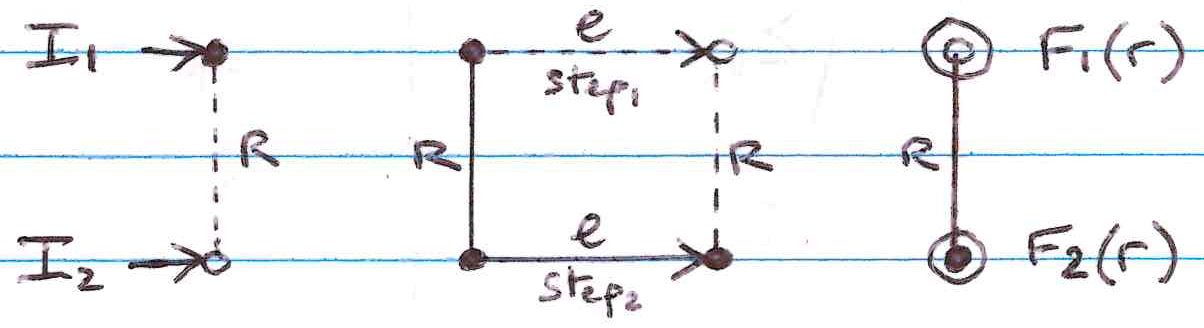
\includegraphics[scale=.65]{figs/bwsim}
\end{center}
This is enough to show that every behavior of the target program
has a corresponding behavior of the source program.

We can compose simulations vertically,
so that Compcert's compilation passes
can be verified one by one.
\end{frame}
%}}}

\section{Expressivity}

\begin{frame}{Interface of Modules} %{{{
Compcert models a whole program with no parameters,
that returns a single integer result.

Instead, we want to expose the various ways in which
the environment can invoke the module
(different functions, argument values, initial memory states),
and the various ways in which the module can return
control to the environment
(return value, new memory state):
\begin{center}
  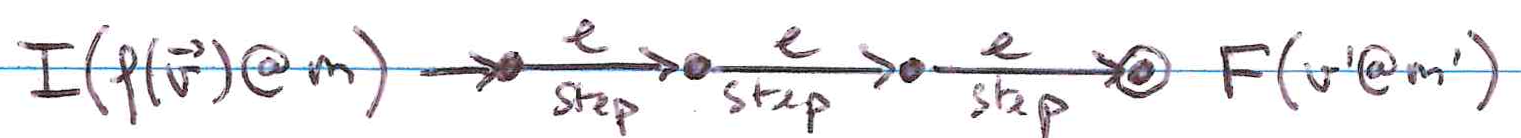
\includegraphics[scale=.65]{figs/comptrsys}
\end{center}
\end{frame}
%}}}

\begin{frame}{External Calls Events} %{{{
Dually, we want the module to be able to
invoke external functions.
We record external calls
as events of the form:
\[
  \kw{extcall}[f(\vec{v})@m, v'@m']
\]

Then we can instantiate
$\kw{external\_functions\_sem}$:
for a given invocation configuration $f(\vec{v})@m$,
we non-deterministically choose
all possible return configurations $v'@m'$
which are valid
(per the behavioral aspects of $\kw{extcall\_properties}$).
\end{frame}
%}}}

\begin{frame}{A problem} %{{{
But wait!

Now we have exposed language-specific values and memories
in our event traces and
in the interface of our transition systems.

We can no longer assume the traces of the source and target
will be exactly the same!
And we need to take into account the language-specific information
used for initial states,
and for the eventual outcome
if the machine ever reaches a final state.
\end{frame}
%}}}

\section{Abstraction}

\begin{frame} %{{{
We need to specify the way in which source values and memory states
relate to target ones:
in essence,
this is the calling convention $\mathbb{R}$
which applies to the pair
of the languages we're trying to relate.

Since Compcert bundles together the notions of
refinement (fewer behaviors) and
abstraction (the behaviors are expressed differently)
into its notion of simulation,
let's call our corresponding construction a
\emph{simulation convention}.
\end{frame}
%}}}

\begin{frame}{Simulation Convention} %{{{
A simulation convention $\mathbb{R}$ specifies:
\begin{itemize}
  \item a set of worlds $W$;
  \item a $W$-indexed relation on call states
    $\mathbb{R}^\kw{q}_w \subseteq (\kw{val}^* \times \kw{mem})^2$
  \item a $W$-indexed relation on return states
    $\mathbb{R}^\kw{r}_w \subseteq (\kw{val} \times \kw{mem})^2$
\end{itemize}
There are three simulation conventions in Compcert:
equality, extensions, injections.
Everything composes into the injection convention in the end.

The simulation convention can encode the relational aspects
of $\kw{extcall\_properties}$.
\end{frame}
%}}}

\begin{frame}{Backward simulations} %{{{
Our events are related if they are equal non-extcall events,
or if they respect the simulation convention:
\[
  \AxiomC{$
    \exists w,
      (\vec{v}_1, m_1) \:[\mathbb{R}^\kw{q}_w]\: (\vec{v}_2, m_2) \wedge
      (v_1', m_1') \:[\mathbb{R}^\kw{r}_w]\: (v_2', m_2')$}
  \UnaryInfC{$
    \kw{extcall}[f(\vec{v}_1)@m_1, v_1'@m_1']
    \sqsupseteq_\mathbb{R}
    \kw{extcall}[f(\vec{v}_2)@m_2, v_2'@m_2']$}
  \DisplayProof
\]
Now we can update our notion of backward simulation:
\begin{center}
  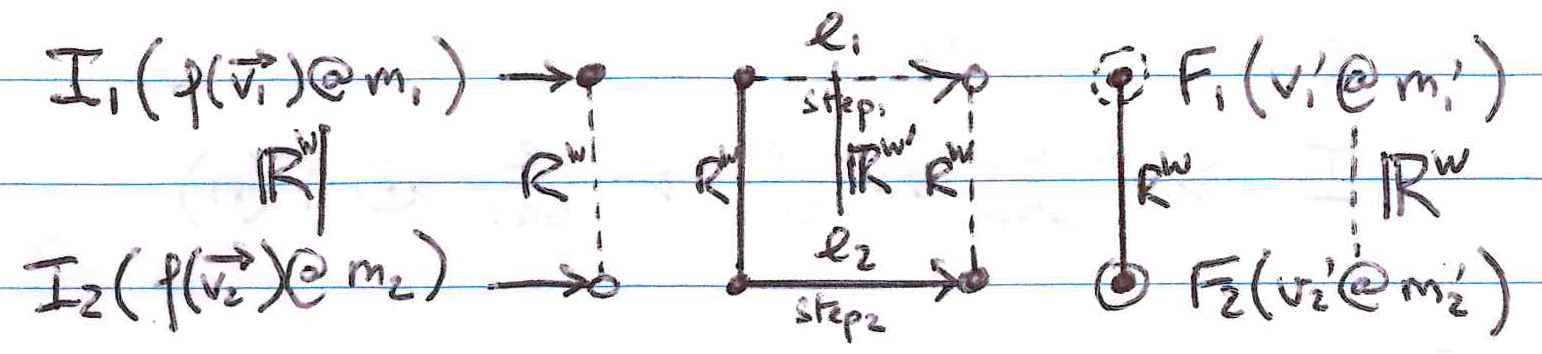
\includegraphics[scale=.65]{figs/bwsimr}
\end{center}
Yay! Our work here is done.
\end{frame}
%}}}

\begin{frame}{Another problem} %{{{
But wait!

Now we have too many target behaviors!

For instance,
assembly can express external calls
which don't respect the C calling convention.

Or, given an external call in the target,
there's no way to know we will have a corresponding
external call in the source.
(Same with final states)
\end{frame}
%}}}

\section{Open Systems}

\begin{frame}{Alternating Simulations} %{{{
This is because for open systems,
we need to use \emph{alternating simulations}:
\begin{center}
  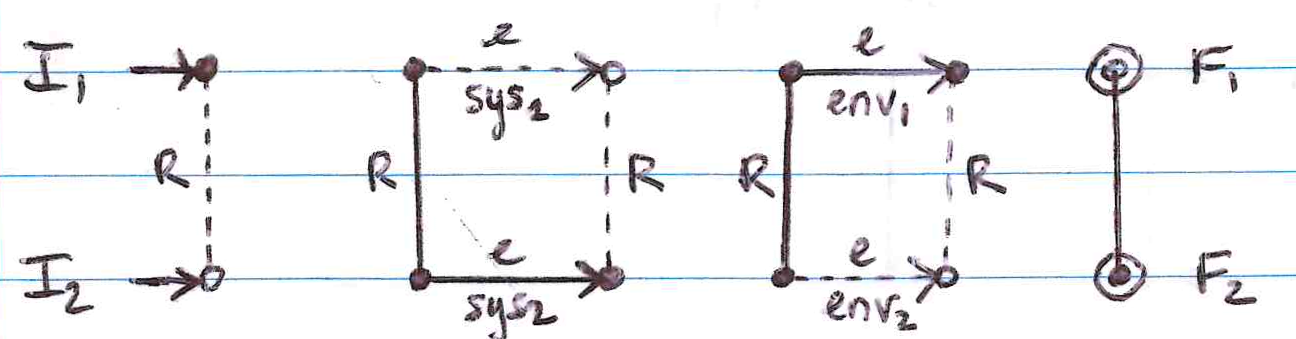
\includegraphics[scale=.65]{figs/altsim}
\end{center}
This is already reflected in Compcert
by the direction of the simulation for initial states
(an environment action).

But otherwise not an issue in vanilla Compcert
because languages are receptive:
they must handle \emph{all} possible environment
behaviors,
and behaviors of the source and target are identical.
\end{frame}
%}}}

\begin{frame}{Half-Steps} %{{{
We want to adapt alternating simulations to Compcert.

Unfortunately,
Compcert does not have distinct \emph{system} and \emph{environment} events.
Instead,
each event denotes both a system action
(request input, call external function),
then an environment action
(function returned $x$, user input was $y$).

So we use an updated $\kw{match\_traces}$ relation
which only compares the system action component and
ignores the environment action component:
\[
  \AxiomC{$
      (\vec{v}_1, m_1) \:[\mathbb{R}^\kw{q}_w]\: (\vec{v}_2, m_2)$}
  \UnaryInfC{$
    \kw{extcall}[f(\vec{v}_1)@m_1, v_1'@m_1']
    \succeq_\mathbb{R}^w
    \kw{extcall}[f(\vec{v}_2)@m_2, v_2'@m_2']$}
  \DisplayProof
\]
\end{frame}
%}}}

\begin{frame}{Alternating simulations for Compcert} %{{{
Now we can replace backward simulation
with Compcert-style alternating relations:
\begin{center}
  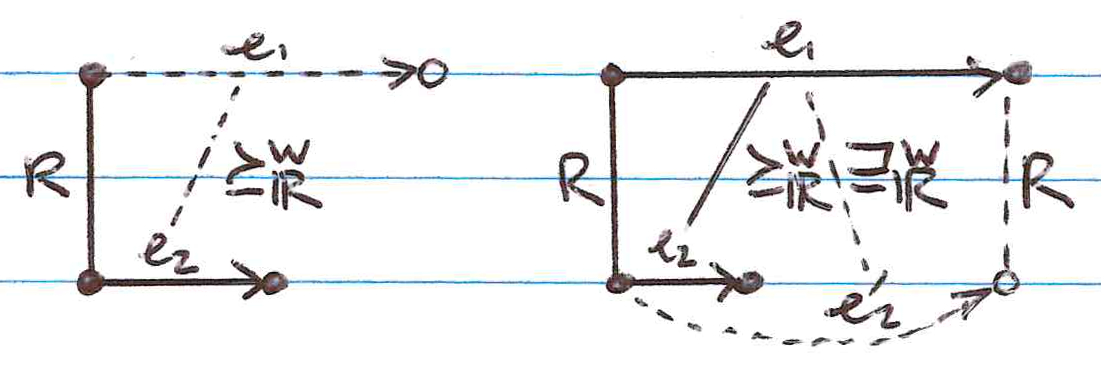
\includegraphics[scale=.65]{figs/altsimc}
\end{center}
\end{frame}
%}}}

\begin{frame}{To make it work\ldots} %{{{
To implement, we need to:
\begin{itemize}
  \item update the meta-theory in Compcert; (medium)
  \item define our simulation conventions,
    show injection absorbs everything; (not that hard)
  \item show compatibility in each pass between
    the simulation relation and
    the simulation convention. (easy but many)
\end{itemize}
\end{frame}
%}}}

\section{Compositionality}

\begin{frame}{Horizontal Composition} %{{{
We want to define semantic horizontal composition and show:
\[
  \llbracket M_1 + M_2 \rrbracket \equiv
  \llbracket M_1 \rrbracket \bullet
  \llbracket M_2 \rrbracket
\]
Basically,
substitute some extcall events by executions of the other module.
Keep a stack of continuations
as part of the state,
so that we can resume when that execution is done.
\end{frame}
%}}}

\begin{frame}{Separate Compilation} %{{{
As one application, we can show the Separate Compcert theorem:
\[ \llbracket M_1 + M_2 + \cdots \rrbracket \sqsupseteq_\kw{inj}
   \llbracket C(M_1) + C(M_2) + \cdots \rrbracket \,, \]
from the per-module semantic preservation theorem,
the horizontal composition theorem, and
the monotonicity properties of $\sqsupseteq_\kw{inj}$ and $\bullet$.
\end{frame}
%}}}

\begin{frame}{Semantic Contextual Refinement} %{{{
We can also show the Compositional Compcert ``semantic contextual refinement''
theorem.
For any context $\sigma \sqsupseteq_\kw{inj} \sigma$,
\[
  \sigma \bullet \llbracket M_1 \rrbracket \sqsupseteq_\kw{inj}
  \sigma \bullet \llbracket C(M_1) \rrbracket \,,
\]
from the per-module semantic preservation theorem
and the monotonicity of $\bullet$.
\end{frame}
%}}}

\begin{frame}{CertiKOS layers!} %{{{
If the memory states are instrumented with abstract state,
we can encode CertiKOS layers as a semantic object
and compose them horizontally with the client.
We can do our code and refinement proofs
in that framework too.
We can instantiate \kw{liblayers} to use it.

However memory state is the only way to keep state across calls.
Our transition systems have no memory from one call to the next otherwise.
\end{frame}
%}}}

\begin{frame}{Other things!} %{{{
By constructing ad-hoc machines we can model
fork, IPC, longjmp, etc.

In a richer semantics we could express the behavior
of longjmp as another semantic object to compose with
(instead of an ad-hoc machine operator).
\end{frame}

\end{document}

